\documentclass{sig-alternate}
\usepackage[backend=bibtex,style=numeric-comp]{biblatex}
\usepackage{tikz}

\newcommand{\code}[1]{\texttt{#1}}

\author{
\alignauthor{}
Dan Stelljes\\
  \affaddr{Division of Science and Mathematics}\\
  \affaddr{University of Minnesota, Morris}\\
  \affaddr{Morris, Minnesota, USA 56267}\\
  \email{stell124@morris.umn.edu}
}
\conferenceinfo{UMM CSci Senior Seminar Conference, December 2016}{Morris, MN}
\title{Composable Concurrency Models}

\bibliography{references}

\AtEveryBibitem{\clearfield{doi}}
\AtEveryBibitem{\clearfield{note}}

\begin{document}

\maketitle

\begin{abstract}

The need to manage concurrent operations in applications has led to the development of a variety of concurrency models. Modern programming languages generally provide several concurrency models to serve different requirements, and programmers benefit from being able to use them in tandem. We discuss challenges surrounding concurrency control and examine situations in which conflicts between models can occur. Additionally, we describe attempts to implement concurrency models on top of lower-level concurrency abstractions.

\end{abstract}

\keywords{concurrency, parallelism, concurrency abstraction}

\section{Introduction}

Most interactive computer programs depend on concurrency, the ability to perform different tasks at the same time. A web browser, for instance, might at any point be rendering documents in multiple tabs, transferring files, and handling user interaction. On a lower level, the operating system might be running several other applications, juggling background processes, and responding to events~\cite{Swalens2014}. If every long-running process blocked other processes from proceeding, the system would be effectively unusable.

Concurrency models enable programmers to reason about and describe interactions between concurrent processes. The web browser is a good example of several different models: The user interface layer might rely on an event loop, the rendering process might operate in shared memory, and suggestions from browsing history or a search engine might require parallel collection operations or map-reduce to achieve acceptable performance~\cite{Marr2012}.

Given that an application is likely to make use of more than one concurrency model, programmers would prefer that different models could be combined. Composability is also desirable from an engineering standpoint---a virtual machine for one or more high-level languages should be able to support a variety of models without sacrificing semantics or performance. However, different concurrency models are not necessarily composable and unexpected issues may arise when they interact. Recent work has attempted to identify unifying concurrency abstractions that would guarantee composability of different models and also provide underlying virtual machine support~\cite{Marr2009, Marr2012, Swalens2014, Ziv2015}.

\section{Background}

Modern operating systems are expected to run many processes concurrently, and processes themselves are often composed of multiple concurrent threads of execution. A processor can only execute one thread at a time, so multitasking is accomplished by rapidly switching between threads~\cite{Liu1973}. Although concurrent threads may appear to be executed simultaneously, truly parallel execution can only take place across multiple processors.

Concurrency models can abstract over implementation details, allowing programmers to reason in terms of asynchronous tasks and independent components instead of low-level thread management. In addition to making a program more understandable, higher-level models afford a degree of flexibility: Concurrent operations could be executed in an event loop on one thread, executed in multiple threads on the same processor, or executed in parallel.

\subsection{Concurrency}

For operations to be executed concurrently, they must be able to be executed out of order or in partial order. Lamport, in his foundational work on distributed systems, formalized this by defining a ``happens before'' relation (denoted by ``$\rightarrow$'') on a set of operations: If $A$ and $B$ are operations in the same process and $A$ occurs before $B$, or if $A$ is the sending of a message by one process and $B$ is the receipt of the same message by another process, then $A \rightarrow B$. Two operations $A$ and $B$ are said to be concurrent if $A \nrightarrow B$ and $B \nrightarrow A$~\cite{Lamport1978}.

While the ``happens before'' relation can be used to determine whether operations can be executed concurrently, it does not guarantee the correctness of the results. In a non-concurrent (entirely sequential) program, it would be sufficient to show that the program is correct after the execution of each task and therefore correct upon termination.

\begin{figure}
  \centering
  \begin{tikzpicture}
    \draw [|-|] (0,0) node[left=3pt] {$ x $} -- (6,0);

    \draw [<-] (0.5,0.25) -- (0.5,0.75) node[above=3pt] {$ 1 $};
    \draw [->] (1,0.25) -- (1,0.75) node[above=3pt] {$ 1 $};

    \draw [<-] (2,0.25) -- (2,0.75) node[above=3pt] {$ 2 $};
    \draw [->] (2.75,0.25) -- (2.75,0.75) node[above=3pt] {$ 2 $};
    \draw [->] (3.25,0.25) -- (3.25,0.75) node[above=3pt] {$ 2 $};

    \draw [<-] (3.75,0.25) -- (3.75,0.75) node[above=3pt] {$ 3 $};

    \draw [<-] (4.5,0.25) -- (4.5,0.75) node[above=3pt] {$ 4 $};
    \draw [->] (5.5,0.25) -- (5.5,0.75) node[above=3pt] {$ 4 $};
  \end{tikzpicture}
  \caption{A single thread writes to and reads from a single variable.}
\label{figure:single}
\end{figure}

Figure~\ref{figure:single} illustrates a simple program in which a single thread reads and writes numbers from a variable $x$. (Write operations are denoted by an arrow pointing toward the line and read operations by an arrow pointing away.) The program satisfies an intuitive model of how variables should behave---each time $x$ is read, the value is equal to the value of the most recent write.

\begin{figure}
  \centering
  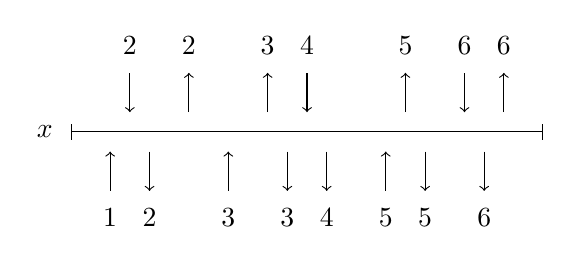
\begin{tikzpicture}
    \draw [|-|] (0,0) node[left=3pt] {$ x $} -- (6,0);

    \draw [<-] (0.5,-0.25) -- (0.5,-0.75) node[below=3pt] {$ 1 $};

    \draw [<-] (0.75,0.25) -- (0.75,0.75) node[above=3pt] {$ 2 $};
    \draw [->] (1,-0.25) -- (1,-0.75) node[below=3pt] {$ 2 $};
    \draw [->] (1.5,0.25) -- (1.5,0.75) node[above=3pt] {$ 2 $};

    \draw [<-] (2,-0.25) -- (2,-0.75) node[below=3pt] {$ 3 $};
    \draw [->] (2.5,0.25) -- (2.5,0.75) node[above=3pt] {$ 3 $};
    \draw [->] (2.75,-0.25) -- (2.75,-0.75) node[below=3pt] {$ 3 $};

    \draw [<-] (3,0.25) -- (3,0.75) node[above=3pt] {$ 4 $};
    \draw [->] (3.25,-0.25) -- (3.25,-0.75) node[below=3pt] {$ 4 $};

    \draw [<-] (4,-0.25) -- (4,-0.75) node[below=3pt] {$ 5 $};
    \draw [->] (4.25,0.25) -- (4.25,0.75) node[above=3pt] {$ 5 $};
    \draw [->] (4.5,-0.25) -- (4.5,-0.75) node[below=3pt] {$ 5 $};

    \draw [<-] (5,0.25) -- (5,0.75) node[above=3pt] {$ 6 $};
    \draw [->] (5.25,-0.25) -- (5.25,-0.75) node[below=3pt] {$ 6 $};
    \draw [->] (5.5,0.25) -- (5.5,0.75) node[above=3pt] {$ 6 $};
  \end{tikzpicture}
  \caption{Two threads concurrently write to and read from a single variable.}
\label{figure:multiple}
\end{figure}

In a concurrent program, the history of operations (that is, the sequence in which operations are executed) may not be the same for every execution. As a result, assumptions about correctness that are true for a sequential program may be violated in a concurrent program. This is illustrated in Figure~\ref{figure:multiple}, in which two threads concurrently write from and read to a variable $x$ concurrently. Because the operations of the threads are interleaved, a read operation on $x$ may not yield a value that matches the value of that thread's most recent write. The value may even be inconsistent between consecutive reads. (Errors that arise due to unintentional dependency on execution order are referred to as race conditions.) From the perspective of a single thread, the program appears to be incorrect because it violates the same intuitive model of how variables should behave.

Consistency models guarantee the correctness of a program by defining a set of all allowed histories. If an execution of a program follows an allowed history, the execution is consistent. If not, the execution is inconsistent. If every possible execution of the program follows an allowed history, the program conforms to the consistency model.

\subsection{Linearizability}

Linearizability (also referred to as atomicity or indivisibility) is a guarantee that the completion of a task will appear to be instantaneous. In other words, a task will take effect atomically at some point during its execution. Any subsequent operation, then, will only see the updated state.

\subsection{Serializability}

Explanation of execution order as a requirement for correctness.

\subsection{Visibility}

Explanation of thread opacity and communication.

\section{Common concurrency models}

\subsection{Atomic variables}

Atomic variables can only be read and mutated by operations that guarantee atomicity. For example, the \emph{compare-and-swap} operation compares the current value of the variable to a given value and only performs a write if the values match. \emph{compare-and-swap} ensures that a new value cannot be based on outdated information. Suppose that a thread $A$ reads a variable $v$ and begins computing a new value. At the same time, another thread $B$ modifies $v$. When $A$ tries to set the value of $v$ via \emph{compare-and-swap}, the write will fail. As a result, all writes on $v$ are guaranteed to be atomic.

\subsection{Software transactional memory}

Software transactional memory (STM) allows multiple concurrent operations to transactionally write to a shared location in memory. STM is an example of optimistic concurrency control: Each operation writes to the shared memory with no regard to the activity of other threads. After the entire transaction is completed, the transaction manager verifies that other threads have not also made changes to the shared memory. If there are conflicting changes, the transaction is aborted and re-executed until it eventually succeeds~\cite{Shavit1995}.

Conceptually, STM simplifies concurrency because it allows transactions to be thought of as a single-threaded operation. A thread cannot observe changes made to other threads while a transaction is in progress, nor can other threads observe modifications by that thread until the transaction is completed. Only when a transaction completes successfully will changes will become visible to other threads.

Harris and Fraser proposed the use of critical regions to represent transactions~\cite{Harris2014}.

\subsection{Communicating threads}

Instead of sharing memory, some concurrency models restrict operations to private memory. Threads communicate strictly by message passing, which avoids race conditions. Communicating sequential processes (CSP), one of the oldest communicating thread models, describes systems in terms of independent processes that communicate through predefined channels~\cite{Hoare1978}.

Other models, most notably the actor model, rely on asynchronous message passing to specific entities~\cite{Agha1986}. Actors can only communicate via asynchronous message passing. Upon receiving a message, an actor can choose to send messages to other actors, create new actors, and determine the behavior used for the next received message.

\subsection{Proxies}

Proxies are placeholders for values that are the result of some concurrently executed operation. Futures and promises are the two main types of proxy, though the terms are frequently used interchangeably (along with ``delayed'' and ``deferred''). Specifically, futures are resolved to the result of the completed operation. The result is then accessed implicitly; any use of the future will return its value. Promises can be created independently and require the result to be accessed explicitly.

\section{Correctness criteria}

\subsection{Safety}

Definition of safety as a guarantee of partial correctness (``nothing bad will happen'').

\subsection{Liveness}

Definition of liveness as a guarantee of progress and eventual termination (``something good will eventually happen'').

\section{Proposed abstractions}

More sources here would be good---Marr and D'Hondt~\cite{Marr2012} provide the only solid abstraction.

\subsection{Asynchronous events}

Ziarek et al.~\cite{Ziarek2011} introduce asynchronous events as a possible abstraction. Their examples are heavily tied to Concurrent ML and might be difficult to integrate.

\subsection{Ownership-based meta-object protocol}

Marr and D'Hondt~\cite{Marr2012} proposed an ownership-based meta-object protocol with the goal of providing VM support. They also demonstrate implementation of actors, STM, agents, and CSP.

\printbibliography{}

\end{document}
